%%%
% Plantilla de Trabajo
% Modificación de una plantilla de Latex de Frits Wenneker para adaptarla 
% al castellano y a las necesidades de escribir informática y matemáticas.
%
% Editada por: Mario Román
%
% License:
% CC BY-NC-SA 3.0 (http://creativecommons.org/licenses/by-nc-sa/3.0/)
%%%

%%%%%%%%%%%%%%%%%%%%%%%%%%%%%%%%%%%%%%%%
% Short Sectioned Assignment
% LaTeX Template
% Version 1.0 (5/5/12)
%
% This template has been downloaded from:
% http://www.LaTeXTemplates.com
%
% Original author:
% Frits Wenneker (http://www.howtotex.com)
%
% License:
% CC BY-NC-SA 3.0 (http://creativecommons.org/licenses/by-nc-sa/3.0/)
%
%%%%%%%%%%%%%%%%%%%%%%%%%%%%%%%%%%%%%%%%%

%----------------------------------------------------------------------------------------
%	PAQUETES Y CONFIGURACIÓN DEL DOCUMENTO
%----------------------------------------------------------------------------------------

%%% Configuración del papel.
% fourier: Usa la fuente Adobe Utopia. (Comentando la línea usa la fuente normal)
\documentclass[paper=a4, fontsize=11pt, spanish]{scrartcl} 
\usepackage{fourier}

% Centra y formatea los títulos de sección.
% Quita la indentación de párrafos.
\usepackage{sectsty} % Allows customizing section commands
\allsectionsfont{\centering \normalfont\scshape} % Make all sections centered, the default font and small caps
\setlength\parindent{0pt} % Removes all indentation from paragraphs - comment this line for an assignment with lots of text

% Permite elegir cabeceras y pies de página.
\usepackage{fancyhdr} % Custom headers and footers
\pagestyle{fancyplain} % Makes all pages in the document conform to the custom headers and footers
\fancyhead{} % No page header - if you want one, create it in the same way as the footers below
\fancyfoot[L]{} % Empty left footer
\fancyfoot[C]{} % Empty center footer
\fancyfoot[R]{\thepage} % Page numbering for right footer
\renewcommand{\headrulewidth}{0pt} % Remove header underlines
\renewcommand{\footrulewidth}{0pt} % Remove footer underlines
\setlength{\headheight}{13.6pt} % Customize the height of the header


%%% Castellano.
% noquoting: Permite uso de comillas no españolas.
% lcroman: Permite la enumeración con numerales romanos en minúscula.
% fontenc: Usa la fuente completa para que pueda copiarse correctamente del pdf.
\usepackage[spanish,es-noquoting,es-lcroman]{babel}
\usepackage[utf8]{inputenc}
\usepackage[T1]{fontenc}
\selectlanguage{spanish}


%%% Matemáticas.
% Paquetes de la AMS. Para entornos de ecuaciones.
\usepackage{amsmath,amsfonts,amsthm}

% Incluye números entre secciones y ecuaciones.
\numberwithin{equation}{section} % Number equations within sections (i.e. 1.1, 1.2, 2.1, 2.2 instead of 1, 2, 3, 4)
\numberwithin{figure}{section} % Number figures within sections (i.e. 1.1, 1.2, 2.1, 2.2 instead of 1, 2, 3, 4)
\numberwithin{table}{section} % Number tables within sections (i.e. 1.1, 1.2, 2.1, 2.2 instead of 1, 2, 3, 4)

%%% Códigos C / C++ / SQL ...
% Paquete listings para visualización de código más elegante
\usepackage{xcolor,listings}
\usepackage{textcomp}
\lstset{upquote=true}

%% Gráficos e imagenes:
\usepackage{graphicx}


%----------------------------------------------------------------------------------------
%	TÍTULO
%----------------------------------------------------------------------------------------
% Título con las líneas horizontales, nombres y fecha.

\newcommand{\horrule}[1]{\rule{\linewidth}{#1}} % Create horizontal rule command with 1 argument of height

\title{
  \normalfont \normalsize 
  \textsc{Universidad de Granada.\\Sistemas Multidimensionales} \\ [25pt] % Your university, school and/or department name(s)
  \horrule{0.5pt} \\[0.4cm] % Thin top horizontal rule
  \huge Seminario práctico 3: \\Introducción a la utilización de una herramienta MOLAP \\ % The assignment title
  \horrule{2pt} \\[0.5cm] % Thick bottom horizontal rule
}

\author{Daniel López García\\Rafael Nogales Vaquero} % Your name

\date{\normalsize\today} % Today's date or a custom date



%----------------------------------------------------------------------------------------
%	DOCUMENTO
%----------------------------------------------------------------------------------------


\begin{document}
\maketitle % Escribe el título
Objetivo: Implementar una base de datos MOLAP y saber realizar operaciones multidimensionales sobre ella para la obtención de informes.\\

\textbf{1. De forma tutelada, realizad las acciones necesarias para implementar, de manera coherente con el diseño conceptual y la base de datos aportada, un cubo multidimensional utilizando la herramienta Excel (Sugerencia: antes de implementar algo con Excel, haced con Access las modificaciones necesarias). Haciendo uso de Excel, cread una tabla dinámica asociada al cubo y obtened, de forma tutelada, el siguiente informe: “Importe de las ventas y cantidad de clientes para cada autor y región de ventas en los primeros siete días del mes de septiembre de 2010”.
Para cada paso realizado en la obtención del informe, indicad la operación que se realiza y el cubo que se obtiene (detallando el nivel en cada una de la dimensiones).Incluid una copia de la pantalla donde se pueda ver el informe final generado.}\medskip

En primer lugar desde Datos->Informe de tablas y datos dinámicos añadimos la base de datos de Access, añadiendo la tabla $consultaExcel$ y creando un cubo OLAP. Durante la creación del cubo añadimos las dimensiones teniendo en cuenta que cada jerarquía debe ser tratada como una dimensión(la dimensión Qué tiene las jerarquías Qué1(Título,Autor) y Qué2(Título,Categoría)). Una vez creada la tabla dinámica, agregamos el autor en el área de filas que es una operación drill-down. El nivel del cubo es Que:Autor, Donde:Todo, Cuando:Todo. A continuación, agregamos la región de ventas en el área de columnas. De nuevo es una operación drill-down y el nivel del cubo es Que:Autor, Donde:Region\_Ventas, Cuando:Todo. Finalmente agregamos la fecha en área de columnas y seleccionamos las fechas indicadas. La operación realizada al seleccionar las fechas es slice\&dice y el nivel del cubo no varía.
\newline
El resultado del informe se muestra en la siguiente imagen:
\begin{center}
	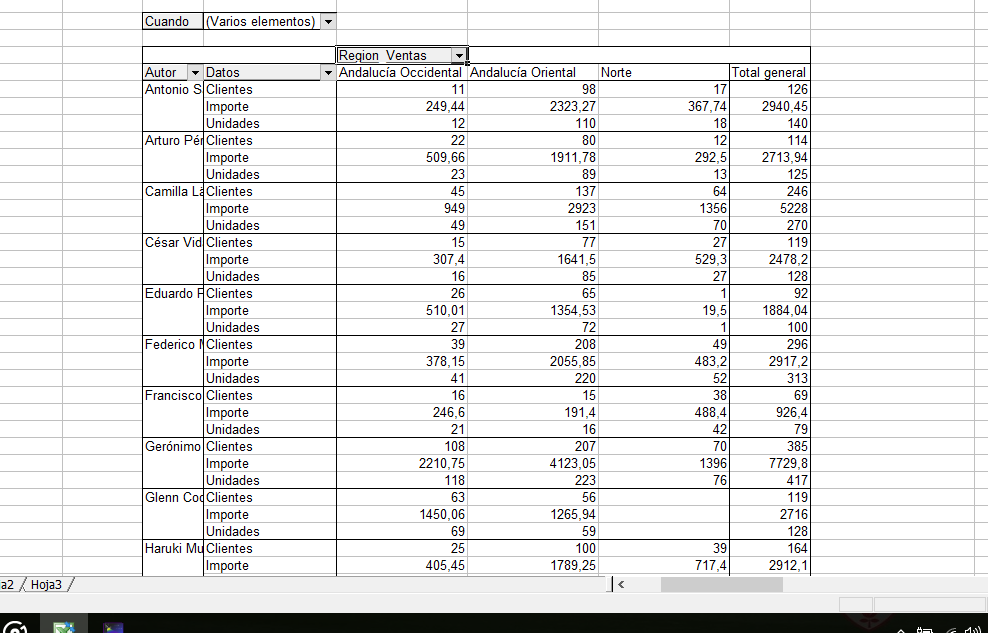
\includegraphics[scale=0.5]{img1.png}
\end{center}
\bigskip
\textbf{2. A partir del informe anterior, definid y obtened con Excel otro informe libre aplicando al menos una vez cada una de las operaciones multidimensionales, indicando, paso a paso, la operación que se aplica y el cubo obtenido en cada caso.
Incluid una copia de la pantalla donde se pueda ver el informe final generado.}\medskip

Ahora queremos ver cuales son los autores preferidos en la zona norte (en la primera semana de Septiembre de 2010), para ello vamos a ver cuántos clientes tiene cada autor y cuantos ejemplares se venden (desglosado por tiendas del norte de España).\\

%Que:Autor, Donde:Region\_Ventas, Cuando:Todo.
En primer lugar hacemos una operacón roll-up sobre las mediciones, vamos a eliminar la medición "importe".
Aunque el nivel del cubo no varía ya que es una operación sobre las mediciones.\\
Lo siguiente que hacemos es una operación drill-down que consiste en añadir tiendas al area de columnas por lo que el nivel del cubo es:  Que:Autor, Donde:Tienda, Cuando:Todo.
Por último vamos a hacer una operación slice\&dice que consiste en seleccionar "Norte" en la región de ventas del área de columnas, el nivel del cubo no varía.\\

El resultado del informe se muestra en la siguiente imagen:
\begin{center}
	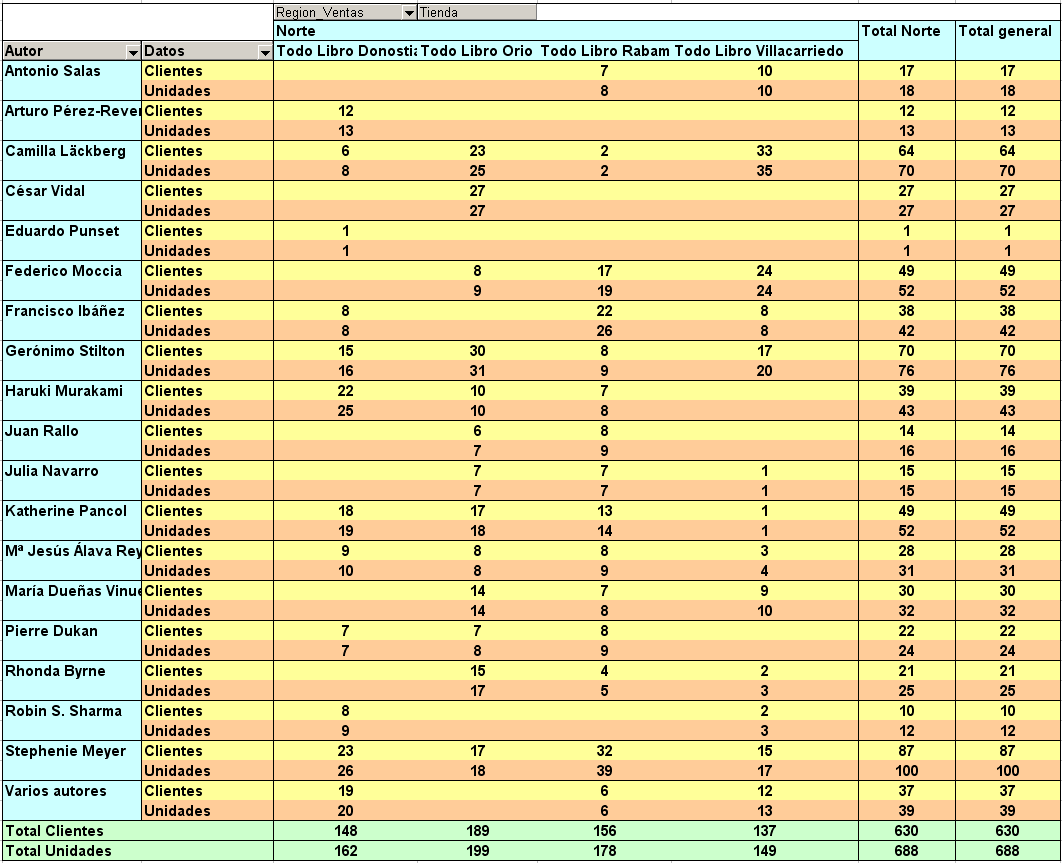
\includegraphics[scale=0.42]{img2.png}
\end{center}




\end{document}